% ---------
%  Compile with "pdflatex hw0".
% --------
%!TEX TS-program = pdflatex
%!TEX encoding = UTF-8 Unicode
%!TEX spellcheck = English (Aspell)

\documentclass[11pt]{article}
\usepackage{jeffe,handout,graphicx}
\usepackage[utf8]{inputenc}		% Allow some non-ASCII Unicode in source

% =========================================================
%   Define common stuff for solution headers
% =========================================================
\Class{Inheritance}
\Semester{c++}
\Authors{1}
\AuthorOne{Jorge Velez}{}
% \AuthorTwo{Friday Caliban}{fcaliban}
% \AuthorThree{Duncan Quagmire}{dquagmir}
\Section{}

% =========================================================
\begin{document}

% ---------------------------------------------------------


\HomeworkHeader{1}{2}	% homework number, problem number

When we look at classes we need a way to define a relationship between other classes and more formally we define 
\emph{inheritance} as a relationship between classes where the class being inherited is the \textbf{\emph{parent class, base class, super class}}, and
the class that is inherited is the \textbf{\emph{child class, derived class, or subclass}}.

\newpage

\begin{solution}
These are, without exception, inappropriate inquiries, a phrase which here means “all the wrong questions”.  Here are the questions you should have asked instead:
\begin{enumerate}[(a)]
\item Why would someone say something was stolen when it was never theirs to begin with?
\item How could someone who was missing be in two places at once?
\item Why would someone destroy one building when they really wanted to destroy another?
\end{enumerate}
\end{solution}

\begin{solution}
Pietrisycamollaviadelrechiotemexity!\footnote{In previous semesters, this would have been worth 25\% partial credit, but no longer.}
\end{solution}

\begin{Sources}
Sunny Baudelaire, Thursday Caliban, Isadora Quagmire, The Henchperson of Indeterminate Gender, Lemony Snickett
\end{Sources}


% ---------------------------------------------------------
% Change authors for all future solutions
\AuthorOne{Marceline Abadeer}{vampireq}
\AuthorTwo{Finn Mertens}{thehuman}
\AuthorThree{Simon Petrikov}{iceking}

\HomeworkHeader{1}{1}	% Problems don’t have to be in order

\newtheorem{lemma}{Lemma}

\begin{solution}[R. Rotten]
Alright! I can see that I will have to teach you how to be \emph{villains!}

\begin{enumerate}[(a)]
\item
Now listen closely.  Here's a little lesson in trickery.  This is going down in history.
If you wanna be a Villain Number One, you have to chase a superhero on the run.  Just follow my moves, and $^{\emph{sneak}}$ around.  Be careful not to make a sound!
Shh!  No, don't touch that!
\[
	\emph{We} = \#1^\text{Hey!}
\]

\item~
\begin{algo}
	\textul{\textsc{HaHaHa}(\emph{net}):}\+
\\	$\emph{net}.\emph{found} \gets \emph{now}$
\\	$\textsc{LookAt}(\emph{net})$
\\	in parallel:\+
\\		for $i\gets 1$ to $100$\+
\\			if $\emph{said\_go} = \textsc{True}$\+
\\				$\emph{net}.\emph{ReadyToThrow} \gets \textsc{True}$\-\-
\\		$\emph{said\_go} \gets \textsc{True}$\-
\\[0.5ex]
	if \emph{net}.\emph{ReadyToThrow}\+
\\		$\textsc{Throw}(\emph{net}, \emph{him}, \lnot me)$\-
\\	\textsc{Try}(\emph{banana}.\emph{peel})
\end{algo}

\begin{algo}
	\textul{$\textsc{Try}(\emph{somethingelse})$:}\+
\\	$\textsc{Watch}(\,)$
\\	$\textsc{Learn}(\,)$
\\	$\emph{deal}.\emph{location} \gets \emph{here}$
\\	return $\textsc{Slip}(\emph{somethingelse}) \land
				\textsc{Slide}(\emph{somethingelse})$
\end{algo}

$\mathsc{HaHaHa}(\emph{Gasp!})$   What are you \emph{doing!?}

\item
Ba-ba-biddly-ba-ba-ba-ba, ba-ba-ba-ba-ba-ba-ba, we are number one. Hey!\\
Ba-ba-biddly-ba-ba-ba-ba, ba-ba-ba-ba-ba-ba-ba, \textbf{VILLAIN NUMBER ONE!}

\item
Ba-ba-biddly-ba-ba-ba-ba, ba-ba-ba-ba-ba-ba-ba, we are number one. Hey!\\
Ba-ba-biddly-ba-ba-ba-ba, ba-ba-ba-ba-ba-ba-ba, we are number one. Hey!\\
We are number one, hey!  We are number one!  We are number one!  Hey! Hey!
\end{enumerate}
\end{solution}

\begin{Sources}~
\begin{itemize}
\cramped % reduce space between bullets
\item
Collaborated with Bonnibel “Stephanie” Bubblegum, Sportacus, and Prismo
\item
\href{https://genius.com/Lazy-town-we-are-number-one-lyrics}{Genius Lyrics}
\item
\emph{Enchiridion}, Chapter 13
\end{itemize}
\end{Sources}


% ---------------------------------------------------------
% Change authors again ; you can omit this if the authors aren’t changing.
\AuthorOne{Anathema Device}{anathema}
\AuthorTwo{Newton Pulsifer}{newt}
\AuthorThree{Adam Young}{ntchrist}

\HomeworkHeader{1}{3}	% homework number, problem number


\begin{solution}
Let $n$ be an arbitrary non-negative integer. There are four cases to consider:
\begin{itemize}
\item
Makin’ pancakes, makin’ bacon pancakes

\item
Make some bacon and I put it in a pancake

\item
Bacon pancakes, that’s what it’s gonna make

\item
\reflectbox{\raisebox{-0.5\height}{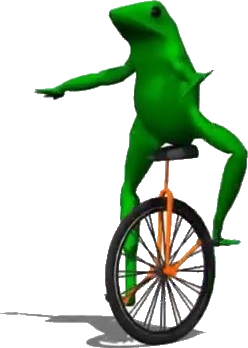
\includegraphics[scale=0.2]{Fig/datboi}}}
\raisebox{-0.5\height}{
\includegraphics[scale=0.4]{Fig/pancakes2}}
\raisebox{-0.5\height}{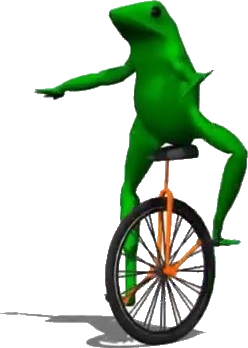
\includegraphics[scale=0.2]{Fig/datboi}}

\end{itemize}
O shit waddup
\end{solution}

\begin{Sources}~
\begin{itemize}
\item
“Is That You?”, \emph{Adventure Time}, Season 6, Episode 19, 2014.
\item
\href{https://sephardicu.com/midrash/frog-or-frogs/}{Midrash on Exodus 8:2}
\item
Collaborated with Hastur,  Jake the Dog, and Dat Boi.
\end{itemize}
\end{Sources}



\end{document}
